\documentclass[runningheads]{llncs}

\usepackage[T1]{fontenc}
\usepackage{lmodern}
\usepackage{graphicx}
\graphicspath{{images/}{./}}
\usepackage{tikz}
\usetikzlibrary{shapes,arrows.meta,positioning,calc,shadows.blur}

\definecolor{pipeBlue}{HTML}{2C6E9E}
\definecolor{pipeBlueLight}{HTML}{EAF3FA}
\definecolor{pipeNavy}{HTML}{1B4965}
\definecolor{pipeNavyLight}{HTML}{D7E6EE}
\definecolor{inGray}{HTML}{555555}
\definecolor{inGrayLight}{HTML}{F2F2F2}
\definecolor{actGreen}{HTML}{2E8B57}
\definecolor{actGreenLight}{HTML}{E7F5EC}
\definecolor{distOrange}{HTML}{D2691E}
\definecolor{distOrangeLight}{HTML}{FBEBDD}

\usepackage{booktabs}
\usepackage{multirow}
\usepackage{amsmath}
\usepackage{amssymb}
\usepackage{hyperref}
\usepackage{array}
\usepackage{algorithm}
\usepackage{algpseudocode}
\usepackage[table]{xcolor}

% Disable automatic hyphenation so words are never broken across a
% line end — a word that doesn't fit moves to the next line whole.
\usepackage[none]{hyphenat}
\sloppy

\begin{document}

\title{Benchmarking Activity and Distortion Classification on Authentically
Distorted Surveillance Videos Using Handcrafted Trajectory Features}

\titlerunning{Classification Benchmarking on Authentically Distorted Surveillance Videos}

\author{Author Name Removed for Review}
\institute{Institution Removed for Review}

\maketitle

% ============================================================
\begin{abstract}
Activity recognition has become a core component of automated 
surveillance systems, yet real-world surveillance footage is 
frequently affected by authentic camera distortions, such as 
defocus blur and exposure variation, that are rarely represented 
in existing benchmarks. Although the Authentically Distorted 
Surveillance Videos (AD-SVD) dataset was introduced for evaluating 
object tracking under these conditions, its suitability for 
supervised classification has not previously been explored. This 
paper reformulates AD-SVD as a benchmark for supervised 
classification by introducing activity recognition and distortion 
classification tasks together with a comprehensive evaluation of 
traditional machine learning classifiers. We show that foreground 
detection, rather than classifier selection, is the primary bottleneck 
limiting downstream performance, with a fixed-threshold detector 
recovering usable trajectories from only 46.5\% of the dataset. 
To address this limitation, we propose a confidence-driven adaptive 
foreground detection method combined with handcrafted trajectory-based 
feature representations. Evaluated using stratified 5-fold cross-validation, 
the proposed approach increases trajectory recovery to 99.7\% of the 
dataset and achieves 75.5\% $\pm$ 0.7 activity recognition accuracy 
and 97.7\% $\pm$ 0.5 distortion classification accuracy using LightGBM, 
outperforming the strongest fixed-threshold baseline. An ablation 
study further shows that improved preprocessing and richer feature 
representations alone cannot account for these gains without adaptive 
foreground detection. This work establishes AD-SVD as a reproducible 
benchmark for activity and distortion classification and demonstrates 
that improving trajectory recovery is fundamental to reliable 
recognition under authentic surveillance distortions.

\end{abstract}



\keywords{
Video Surveillance
\and Activity Recognition
\and Authentically Distorted Surveillance Videos
\and Machine Learning
}

% ============================================================
\section{Introduction}

The growth of public surveillance infrastructure has created a 
fundamental mismatch between the volume of video produced and 
the capacity of human operators to monitor it effectively. 
Fatigue, attention lapses, and delayed response reduce the 
reliability of manual surveillance at scale~\cite{article,ahmed2018trajectory}, 
motivating automated activity recognition as a core capability of intelligent 
surveillance systems.

Although deep learning has achieved impressive performance on large-scale 
action-recognition benchmarks~\cite{ur2023use,xiao2016overview}, its dependence 
on extensive labelled datasets, high computational requirements, and limited 
interpretability continue to present practical challenges for resource-constrained 
deployments~\cite{csurka2018handcrafted,arias2018deep}. Classical handcrafted 
representations remain attractive because they provide transparency, computational 
efficiency, and strong performance in data-constrained settings, but their 
effectiveness depends critically on reliable foreground extraction, making 
them vulnerable to authentic camera distortions such as defocus blur and exposure 
variation, which degrade the edge contrast and luminance information required by 
background subtraction algorithms~\cite{gillani2025distortion}.

Most existing activity-recognition benchmarks are collected under comparatively 
clean recording conditions and therefore provide limited insight into how authentic, 
in-capture distortions affect downstream recognition performance. 
Gomez-Nieto et al.~\cite{9698081} addressed this from the perspective of object 
tracking by introducing the Authentically Distorted Surveillance Videos (AD-SVD) 
dataset, evaluating state-of-the-art trackers under real defocus blur and exposure 
distortions; however, its potential as a benchmark for supervised classification 
has not previously been explored. Establishing classification baselines on 
authentically distorted footage is important because it lets future methods be 
evaluated under realistic deployment conditions rather than idealized laboratory 
environments.

To address this gap, we reformulate AD-SVD as a benchmark for supervised activity 
recognition and distortion classification. Specifically, we investigate whether 
handcrafted trajectory representations retain sufficient discriminative information 
for reliable activity recognition after authentic distortion has degraded foreground 
detection, and whether the same motion representations also encode enough information 
to distinguish distortion types without requiring explicit image-quality analysis. 
Underlying both questions is a working hypothesis: that under authentic distortion, 
the quality of foreground detection, not the choice of classifier or the richness 
of the feature set, sets the ceiling on downstream classification accuracy. The 
remainder of the paper tests this hypothesis directly.

The contributions of this paper are: (i) reformulating AD-SVD as a supervised 
classification benchmark with activity recognition and distortion classification 
tasks; (ii) providing the first comprehensive comparison of traditional machine 
learning classifiers (Random Forest, LightGBM, XGBoost, SVM, and KNN) on this 
dataset; (iii) testing the hypothesis above through a controlled comparison of 
detection, preprocessing, and feature configurations; (iv) proposing a 
confidence-driven adaptive foreground detection strategy that increases trajectory 
recovery to 99.7\% and substantially improves classification performance, with its 
contribution isolated through ablation; and (v) establishing handcrafted trajectory 
representations as a competitive, data-efficient baseline for AD-SVD at its current 
scale, while motivating future comparisons with end-to-end deep learning as larger 
datasets become available.

The rest of the paper follows this plan. Section~2 reviews related work. Section~3 
describes the proposed classification pipeline, including the adaptive detection 
component. Section~4 presents the experimental design and research questions. 
Section~5 answers each research question in turn and discusses implications. 
Section~6 concludes and outlines future work.

% ============================================================
\section{Related Work}

Automated surveillance has long relied on motion analysis to recognise human activities, 
with early approaches primarily based on handcrafted representations derived from 
trajectories, silhouettes, optical flow, and spatio-temporal descriptors. These methods 
remain attractive because they are computationally efficient, interpretable, and require 
substantially less labelled data than modern deep learning approaches, and trajectory-based 
representations in particular have demonstrated competitive performance for surveillance 
applications by effectively capturing human motion patterns while remaining suitable for 
real-time deployment in resource-constrained environments~\cite{ahmed2018trajectory,csurka2018handcrafted}. 
Recent advances in deep learning have significantly improved activity recognition through 
convolutional, recurrent, and transformer-based architectures that learn rich spatio-temporal 
representations directly from video data, achieving state-of-the-art performance on large-scale 
benchmarks, such as UCF101, HMDB51, Kinetics, and Something-Something~\cite{ur2023use,xiao2016overview}. 
Their success, however, generally depends on extensive annotated datasets, considerable computational 
resources, and carefully curated training data, which present practical challenges for surveillance 
applications where labelled data are often limited and deployment constraints favour computationally 
efficient solutions. Consequently, traditional machine learning combined with handcrafted feature 
representations continues to provide a strong and practical baseline for surveillance scenarios 
with limited training data.

Although considerable progress has been made in activity recognition, relatively little attention 
has been devoted to understanding the impact of authentic camera distortions on downstream 
classification performance. Most existing benchmarks either introduce synthetic degradations 
or are collected under favourable recording conditions, limiting their ability to represent 
the challenges encountered by real-world surveillance systems; authentic distortions, 
including defocus blur and exposure variation, degrade foreground quality, fragment object 
trajectories, and consequently reduce the reliability of motion-based feature 
extraction~\cite{gillani2025distortion}. What remains unanswered in this literature is which 
stage of the pipeline actually absorbs that damage: whether the loss is better characterised 
as a classifier-capacity problem, a feature-representation problem, or a detection problem 
upstream of both. Among adaptive background-subtraction methods proposed for challenging 
conditions, including Visual Background Extractor (ViBe), Self-Balanced Sensitivity Segmenter 
(SuBSENSE), and Pixel-Based Adaptive Segmenter (PBAS), we build on MOG2 because it is lightweight, 
widely available, and already the detector against which prior AD-SVD tracking work is 
compared~\cite{9698081}, making it the natural point at which to introduce confidence-driven 
adaptation.

Gomez-Nieto et al.~\cite{9698081} introduced AD-SVD specifically to evaluate object tracking 
algorithms under authentic camera distortions, and their analysis, along with all subsequent 
use of the dataset, has stayed at the tracking level; no prior study has asked whether the 
same detection difficulties that complicate tracking also limit downstream supervised 
classification, or whether classifier choice can compensate for them.

\begin{table}[htbp]
\centering
\caption{Comparison of representative studies and the proposed work.
\textbf{Act.} = Activity Classification; \textbf{Dist.} = Distortion Classification;
\textbf{ML} = Traditional Machine Learning; \textbf{DL} = Deep Learning.
$^{\dagger}$DL used only for tracking, not classification.}
\label{tab:comparison}
\scriptsize
\setlength{\tabcolsep}{1.8pt}
\renewcommand{\arraystretch}{0.95}
\begin{tabular}{@{}l c c c c c c@{}}
\toprule
\textbf{Paper} & \textbf{AD-SVD} & \textbf{Track.} & \textbf{Act.} &
\textbf{Dist.} & \textbf{ML} & \textbf{DL} \\
\midrule
Gomez-Nieto et al.~\cite{9698081} (AD-SVD intro.) &
$\checkmark$ & $\checkmark$ & -- & -- & -- & $\checkmark$$^{\dagger}$ \\
Wang et al.~\cite{wang2012dense} (dense trajectories) &
-- & -- & $\checkmark$ & -- & $\checkmark$ & -- \\
Ahmed et al.~\cite{ahmed2017action} (HOG3D + Random Forest) &
-- & -- & $\checkmark$ & -- & $\checkmark$ & -- \\
Bai and Reibman~\cite{bai2016characterizing} (distortion char.) &
-- & -- & -- & $\checkmark$ & $\checkmark$ & -- \\
\textbf{This work} &
$\checkmark$ & $\checkmark$ & $\checkmark$ & $\checkmark$ & $\checkmark$ & -- \\
\bottomrule
\end{tabular}
\end{table}

Table~\ref{tab:comparison} summarises the relationship between representative 
studies and the present work. Existing research has investigated either activity 
recognition under controlled recording conditions or object tracking under 
authentic surveillance distortions, but rarely their combination within a unified 
classification framework. To the best of our knowledge, this work is the first to 
reformulate AD-SVD as a benchmark for both activity recognition and distortion 
classification while comprehensively comparing multiple traditional machine 
learning classifiers, and to demonstrate that improving foreground detection 
quality is fundamental to reliable downstream classification under authentic 
surveillance distortions.

% ============================================================
\section{Proposed Classification Pipeline}

This section describes the pipeline for transforming raw, authentically distorted 
surveillance videos into activity and distortion predictions. The pipeline is 
formulated as a sequential information transformation, illustrated in 
Figure~\ref{fig:pipeline}:
\[
V \;\xrightarrow{f_{\text{pre}}}\; V'
  \;\xrightarrow{f_{\text{det}}}\; M
  \;\xrightarrow{f_{\text{trk}}}\; \mathcal{T}
  \;\xrightarrow{f_{\text{feat}}}\; \mathbf{x}
  \;\xrightarrow{f_{\text{clf}}}\; (\hat{a},\,\hat{d}),
\]
where $V'$ denotes the preprocessed video, $M$ the foreground-mask sequence, 
$\mathcal{T}$ the set of valid object trajectories, $\mathbf{x}$ the aggregated 
video-level feature vector, $\hat{a}$ the predicted activity class, and $\hat{d}$ 
the predicted distortion class. Because information discarded at one stage cannot 
be recovered later, the pipeline is deliberately structured to test the hypothesis 
raised in Section~1: if foreground detection is the weakest stage, then strengthening 
it, rather than enriching preprocessing, features, or classifier choice downstream, 
should account for most of the achievable gain. Section~3 introduces adaptive 
detection as the mechanism for doing so; Sections~4 and~5 isolate its 
contribution from the other stages.

% Pipeline figure
\begin{figure}[htbp]
\centering
\resizebox{\textwidth}{!}{%
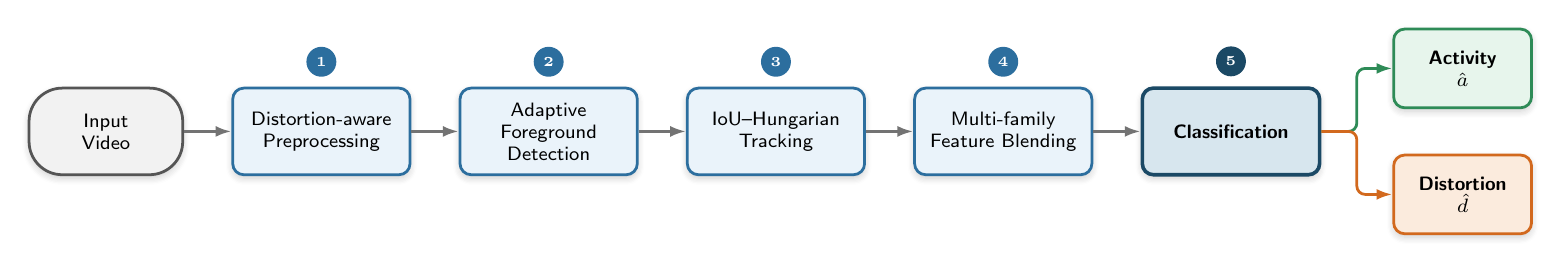
\begin{tikzpicture}[
    node distance=6mm,
    font=\scriptsize\sffamily,
    box/.style={
        draw=pipeBlue,
        line width=1pt,
        rounded corners=4pt,
        fill=pipeBlueLight,
        minimum height=1.1cm,
        text width=1.9cm,
        align=center,
        inner sep=5pt,
        blur shadow={shadow blur steps=6, shadow xshift=0pt,
                    shadow yshift=-1.2pt, shadow blur radius=2.5pt,
                    shadow opacity=20}
    },
    inbox/.style={
        box,
        draw=inGray,
        fill=inGrayLight,
        rounded corners=12pt,
        text width=1.6cm
    },
    finalbox/.style={
        box,
        draw=pipeNavy,
        fill=pipeNavyLight,
        line width=1.3pt,
        font=\scriptsize\sffamily\bfseries
    },
    outboxAct/.style={
        box, draw=actGreen, fill=actGreenLight,
        text width=1.4cm, minimum height=1cm,
        font=\scriptsize\sffamily\bfseries
    },
    outboxDist/.style={
        box, draw=distOrange, fill=distOrangeLight,
        text width=1.4cm, minimum height=1cm,
        font=\scriptsize\sffamily\bfseries
    },
    stepcircle/.style={
        circle, fill=pipeBlue, text=white,
        font=\tiny\bfseries, inner sep=0pt,
        minimum size=3.8mm
    },
    arrowmain/.style={
        -{Latex[length=2mm,width=1.4mm]},
        draw=black!55, line width=1pt
    },
    arrowAct/.style={
        -{Latex[length=2mm,width=1.4mm]},
        draw=actGreen, line width=1pt, rounded corners=3pt
    },
    arrowDist/.style={
        -{Latex[length=2mm,width=1.4mm]},
        draw=distOrange, line width=1pt, rounded corners=3pt
    }
]

% --- nodes ---
\node[inbox] (v) {Input\\Video};

\node[box, right=6mm of v] (pre)
    {Distortion-aware\\Preprocessing};
\node[box, right=6mm of pre] (det)
    {Adaptive Foreground\\Detection};
\node[box, right=6mm of det] (trk)
    {IoU--Hungarian\\Tracking};
\node[box, right=6mm of trk] (feat)
    {Multi-family\\Feature Blending};
\node[finalbox, right=6mm of feat] (clf)
    {Classification};

\node[outboxAct, right=9mm of clf, yshift=8mm]
    (act) {Activity\\$\hat{a}$};
\node[outboxDist, right=9mm of clf, yshift=-8mm]
    (dist) {Distortion\\$\hat{d}$};

% --- step numbers ---
\node[stepcircle, above=1.2mm of pre.north] {1};
\node[stepcircle, above=1.2mm of det.north] {2};
\node[stepcircle, above=1.2mm of trk.north] {3};
\node[stepcircle, above=1.2mm of feat.north] {4};
\node[stepcircle, fill=pipeNavy, above=1.2mm of clf.north] {5};

% --- arrows ---
\draw[arrowmain] (v)   -- (pre);
\draw[arrowmain] (pre) -- (det);
\draw[arrowmain] (det) -- (trk);
\draw[arrowmain] (trk) -- (feat);
\draw[arrowmain] (feat)-- (clf);

\draw[arrowAct]
    (clf.east) -| ($(clf.east)!0.5!(act.west)$) |- (act.west);
\draw[arrowDist]
    (clf.east) -| ($(clf.east)!0.5!(dist.west)$) |- (dist.west);

\end{tikzpicture}%
}
\caption{\textbf{Overview of the proposed classification pipeline.}
Each stage progressively transforms the previous stage's output into a
more compact representation, culminating in classification of both
activity ($\hat{a}$) and distortion ($\hat{d}$).}
\label{fig:pipeline}
\end{figure}

\paragraph{Distortion-aware preprocessing.}

Each video frame is resized to $640\times480$ to provide a consistent 
input resolution while reducing computational cost. Blur is identified 
using the variance of the Laplacian (threshold 100), after which an 
unsharp mask ($\sigma=2.0$, strength 1.5) enhances edge contrast. 
Exposure abnormalities are detected from image intensity statistics 
(lower and upper thresholds of 60 and 195, respectively) and corrected 
using Contrast Limited Adaptive Histogram Equalization (CLAHE) with a 
clip limit of 2.0 and an $8\times8$ tile grid. These operations 
improve local contrast and edge definition before foreground 
extraction while preserving the natural characteristics of the 
recorded distortions.

\paragraph{Confidence-driven adaptive foreground detection.}

Foreground segmentation is performed using MOG2 with a history length 
of 20, a nominal variance threshold $\tau=25$ % TODO(var_threshold sweep): code default is 16; set tau to the value chosen by mog2_threshold_sweep.py and re-run all tables
, and shadow detection 
disabled. Each frame's mask is scored by a mask-quality function 
$Q_{\text{mask}} \in [0,1]$ that combines three measures multiplicatively, 
so that a failure on any single axis collapses the overall score:
\begin{equation}
Q_{\text{mask}} = C \cdot F \cdot S,
\label{eq:maskquality}
\end{equation}
where $C$ is a coverage score peaked around 2\% foreground area, $F$ is a 
fragmentation score that decays linearly once the blob count exceeds 30, 
and $S$ is a resolution-invariant blob-size score. This mask score is 
then combined with an exponential-moving-average track-quality prior 
$Q_{\text{track}}$, updated once per frame from the previous frame's 
tracker output, to give the overall confidence:
\begin{equation}
Q = w \, Q_{\text{mask}} + (1-w) \, Q_{\text{track}}, \qquad w = 0.7.
\label{eq:confidence}
\end{equation}
If $Q$ falls below a threshold of 0.4, detection is re-run at a relaxed 
variance threshold interpolated between $\tau=25$ and a target of 10 in 
proportion to how far below 0.4 the confidence falls, clipped to a safety 
floor of 8, and the re-run mask is kept only if its mask-quality score 
improves on the original (Algorithm~\ref{alg:adaptive}). Morphological 
closing (two iterations) followed by opening (one iteration) removes 
small gaps and isolated noise, while connected components smaller than 
500 pixels are discarded. For brevity we refer to this component as 
Adaptive MOG2 throughout the rest of the paper.

\begin{algorithm}[htbp]
\small
\caption{Confidence-driven Adaptive MOG2 (per frame)}
\label{alg:adaptive}
\begin{algorithmic}[1]
\Require frame $I$, nominal threshold $\tau=25$, relaxed target $\tau_r=10$, floor $\tau_{\min}=8$, confidence threshold $q=0.4$
\State $M \gets \textsc{MOG2}(I, \tau)$; $Q_{\text{mask}} \gets$ score of $M$ (Eq.~\eqref{eq:maskquality})
\State $Q \gets w\,Q_{\text{mask}} + (1-w)\,Q_{\text{track}}$ (Eq.~\eqref{eq:confidence})
\If{$Q \geq q$}
    \State \Return detections from $M$ \Comment{confident — keep}
\Else
    \State $\alpha \gets 1 - Q / q$; \; $\tau' \gets \tau - \alpha(\tau - \tau_r)$, clipped to $[\tau_{\min}, \tau]$
    \State $M' \gets \textsc{MOG2}(I, \tau')$; \; $Q'_{\text{mask}} \gets$ score of $M'$
    \State \Return detections from $M'$ if $Q'_{\text{mask}} > Q_{\text{mask}}$, else from $M$
\EndIf
\end{algorithmic}
\end{algorithm}

\paragraph{Tracking.}

Detected foreground regions are associated across consecutive frames using 
IoU-based matching (threshold 0.3) solved with the Hungarian algorithm; 
tracks may disappear for up to 30 frames before termination, trajectories 
are capped at 300 frames, and those shorter than 30 frames are discarded 
as unreliable, leaving continuous object trajectories suitable for 
feature extraction.

\paragraph{Multi-family feature blending.}

Each surviving trajectory is represented using 221 handcrafted features covering 
trajectory, circular-motion, kinematic, shape, wavelet, and interaction descriptors, 
complemented by appearance features from Histogram of Oriented Gradients (HOG) and 
Local Binary Patterns (LBP) computed independently of tracking success. Mean, 
maximum, and standard deviation statistics are aggregated across all valid 
trajectories into a fixed-length feature vector per video, enabling video-level 
rather than only frame-level classification.

\paragraph{Classification.}

Feature vectors are standardised within a scikit-learn \texttt{Pipeline} to 
prevent information leakage between folds. Five classifiers are evaluated: 
Random Forest (200 trees, balanced class weights), SVM (RBF kernel, $C=10$), 
KNN ($k=5$), LightGBM, and XGBoost (200 estimators, max depth six); a custom 
first-principles Random Forest is evaluated for the baseline configuration only. 
All classifiers use identical stratified five-fold cross-validation splits for 
a fair comparison.

\paragraph{Baseline configuration.}

To quantify the influence of foreground detection on downstream performance, 
a fixed-threshold baseline is evaluated using standard preprocessing, 
conventional MOG2 with a fixed variance threshold of 25, IoU-Hungarian 
tracking, and a 54-dimensional trajectory-only feature 
representation, intentionally conservative rather than artificially weakened. 
A custom Random Forest (information-gain splitting, bootstrap aggregation, 
200 trees, max depth 10) is included here to compare a first-principles 
implementation against well-established libraries.

\paragraph{Preprocessing and feature ablation.}

To isolate adaptive detection from richer preprocessing and features, an 
ablation applies distortion-aware preprocessing and the full 147-dimensional 
feature representation while retaining the same fixed-threshold MOG2 detector 
as the baseline. Comparing this configuration with the proposed pipeline 
isolates the benefit of adaptive detection, while comparison with the 
baseline quantifies the contribution of preprocessing and feature 
enrichment alone.

\paragraph{Why deep learning is not the primary comparison.}

Although end-to-end deep video models represent an important alternative, 
AD-SVD contains only 4,476 videos across eight activity classes, which 
provides relatively limited training data for learning robust spatio-temporal 
representations directly from raw video. In contrast, handcrafted trajectory 
and appearance descriptors encode informative motion characteristics 
explicitly, reducing the amount of labelled data required to learn effective 
classifiers. Consequently, traditional machine learning provides a 
competitive and data-efficient baseline under the current dataset size and 
experimental setting. Section~6 discusses the conditions under which 
comparisons with end-to-end deep learning models would become appropriate.

% ============================================================
\section{Experimental Design}

This section describes the AD-SVD dataset, the experimental
configurations evaluated in this study, the evaluation protocol, and the
research questions addressed in Section~5.

The AD-SVD dataset~\cite{9698081,akyk-7b78-20} contains 4,476 surveillance
videos spanning eight suspicious activity classes recorded under four
authentic distortion conditions (Pristine, Exposure, Focus, and
Exposure+Focus). The videos were captured using four surveillance cameras
across seven locations, providing realistic variations in viewpoint,
scene layout, and imaging conditions. Because the proposed approach is
trajectory-based, videos that fail to produce a valid trajectory after
tracking are excluded from the corresponding classification experiment,
since no trajectory-based descriptors can be extracted from them.

All experiments are evaluated using stratified 5-fold
cross-validation, with identical fold partitions used across all
configurations for a given classification task to ensure fair
comparison. Classification performance is primarily measured using
cross-validation accuracy (mean $\pm$ standard deviation across folds),
while weighted F1-score is reported as a complementary metric to account
for any remaining class imbalance~\cite{sargano2017comprehensive}.

Table~\ref{tab:groups} summarises the three experimental configurations
considered in this study. The baseline establishes the performance of a
conventional fixed-threshold pipeline, the ablation isolates the effect
of distortion-aware preprocessing and richer feature representations
without adaptive detection, and the proposed configuration evaluates the
complete adaptive pipeline. Together, these configurations allow the
contribution of adaptive foreground detection to be separated from
improvements introduced by preprocessing, feature representation, and
classifier selection. More advanced trajectory generation approaches,
such as TFCR-based tracking, are discussed as future work in
Section~6 and are therefore not evaluated in this study.

\begin{table}[htbp]
\centering
\caption{\textbf{Experimental configurations used throughout this study.}
D-A = distortion-aware; ``Feat.'' = feature-vector dimensionality.}
\label{tab:groups}
\resizebox{\textwidth}{!}{%
\fontsize{8}{9.6}\selectfont
\begin{tabular}{@{}l l l l c l@{}}
\toprule
\textbf{Configuration} &
\textbf{Detector} &
\textbf{Preproc.} &
\textbf{Features} &
\textbf{Feat.} &
\textbf{Role} \\
\midrule
Baseline &
MOG2 (fixed) &
Standard &
Trajectory only &
54 &
Baseline reference \\

Ablation &
MOG2 (fixed) &
D-A &
Full (traj.+kin.+shape+\ldots) &
147 &
Isolates preproc./features \\

\textbf{Proposed} &
\textbf{Adaptive MOG2} &
\textbf{D-A} &
\textbf{Full + appearance} &
\textbf{221} &
\textbf{Complete pipeline} \\
\bottomrule
\end{tabular}%
}
\end{table}

Table~\ref{tab:dataset} summarises the composition of AD-SVD using the
two marginal distributions reported by the dataset creators
~\cite{9698081,akyk-7b78-20}: the number of videos per distortion
condition and the number of videos per activity class. The distribution
across distortion conditions is intentionally uneven because pristine
videos serve primarily as a reference set relative to the three
distorted conditions. Since the published dataset documentation does not
provide a joint activity-by-distortion distribution, we report the two
marginal distributions separately rather than reconstructing one.

\begin{table}[htbp]
\centering
\caption{\textbf{AD-SVD composition: videos per distortion condition
(left) and per activity class (right).}~\cite{9698081}}
\label{tab:dataset}
\fontsize{8}{9.6}\selectfont
\begin{tabular}{lr}
\toprule
\textbf{Condition} & \textbf{Videos} \\
\midrule
Pristine        & 160 \\
Exposure        & 1,457 \\
Focus           & 1,409 \\
Exposure+Focus  & 1,450 \\
\midrule
\textbf{Total} & \textbf{4,476} \\
\bottomrule
\end{tabular}
\qquad
\begin{tabular}{lr}
\toprule
\textbf{Activity} & \textbf{Videos} \\
\midrule
Fighting in Group     & 546 \\
Leaving Package       & 564 \\
Passing Out           & 571 \\
Person Pushing Person & 558 \\
Person Running        & 549 \\
Prowl                 & 567 \\
Robbery with Knife    & 562 \\
Walking               & 559 \\
\midrule
\textbf{Total} & \textbf{4,476} \\
\bottomrule
\end{tabular}
\end{table}

Figure~\ref{fig:examples} presents one representative frame for
each of the eight activity classes and each of the four authentic
distortion conditions contained in AD-SVD, providing visual context for
the two classification tasks considered throughout the remainder of the
paper.

\begin{figure}[htbp]
\centering
\setlength{\tabcolsep}{2pt}
\begin{tabular}{@{}cccc@{}}
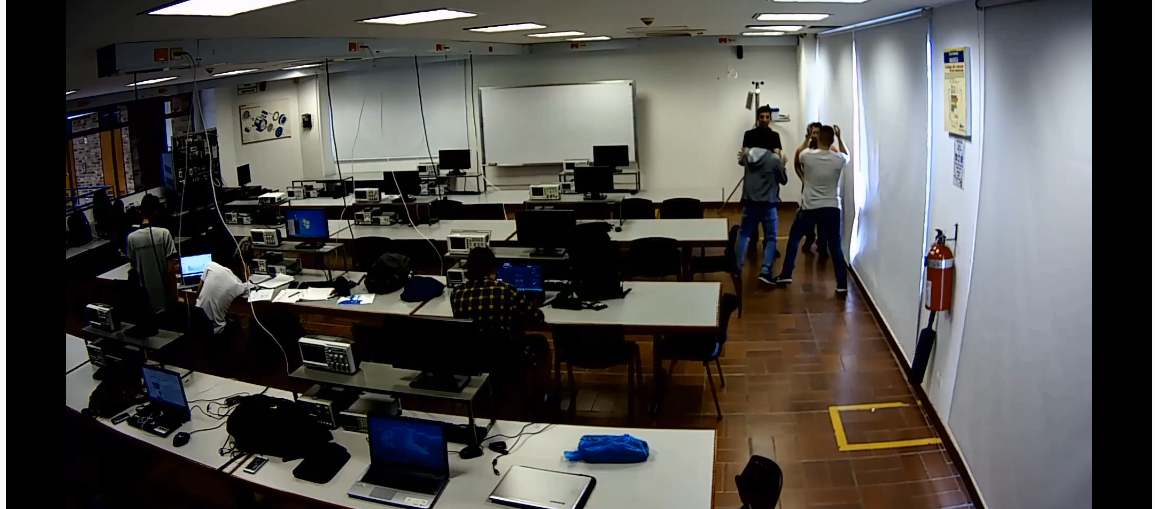
\includegraphics[width=0.19\linewidth]{Fighting_in_Group} &
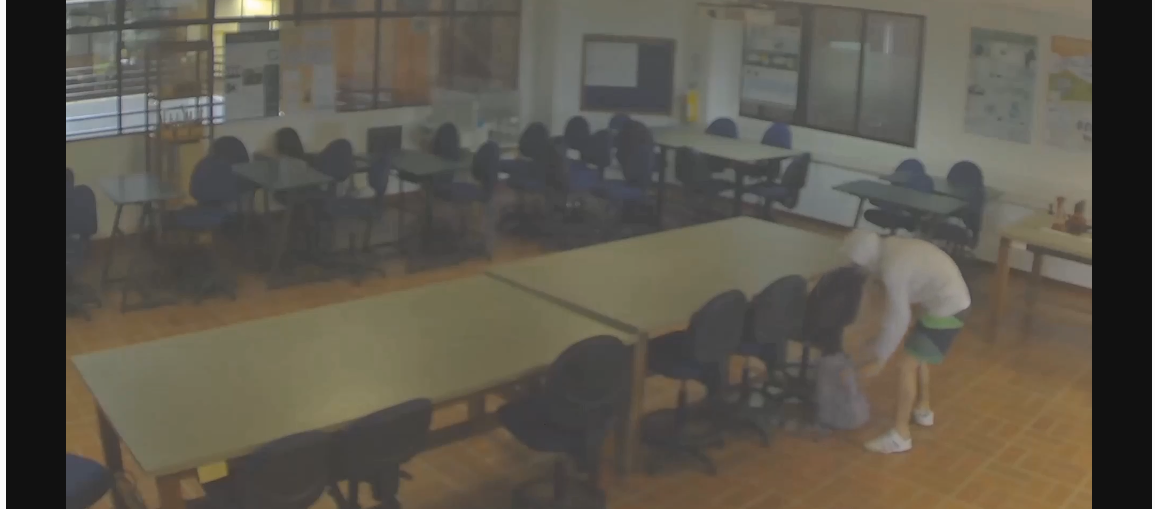
\includegraphics[width=0.19\linewidth]{Leaving_Package} &
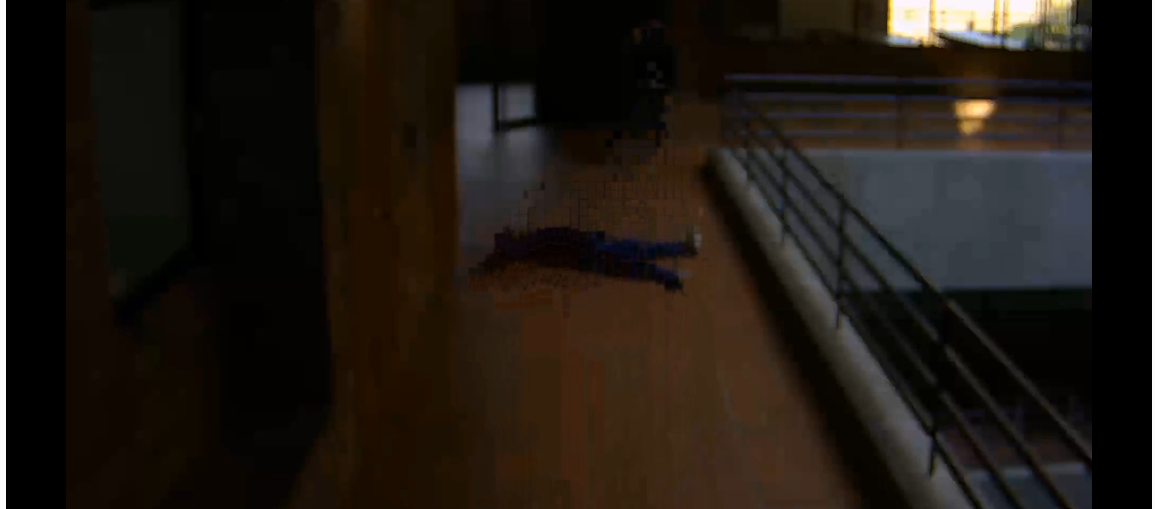
\includegraphics[width=0.19\linewidth]{passing_out} &
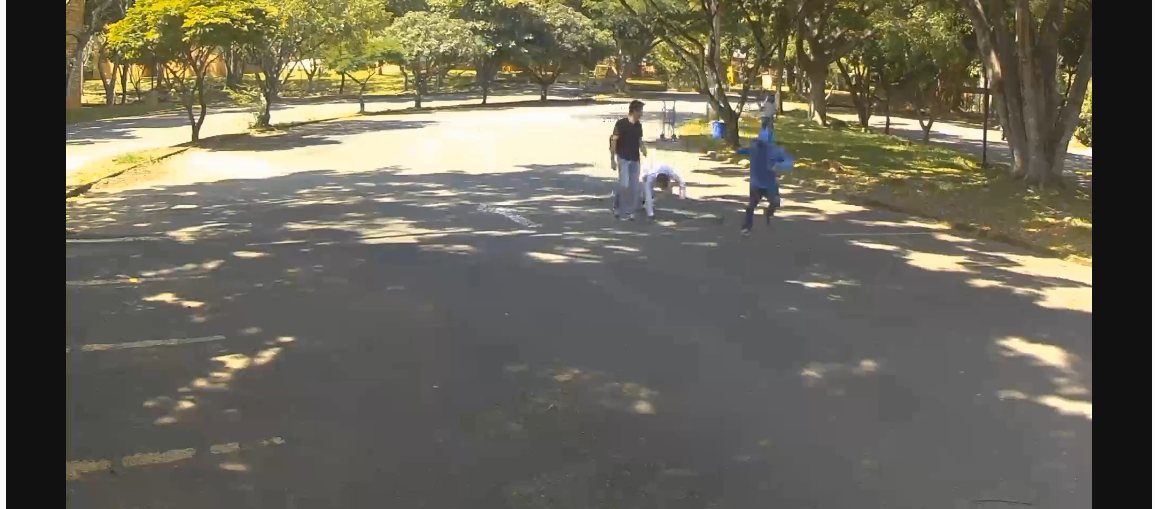
\includegraphics[width=0.19\linewidth]{Person_Pushing_Person} \\
\tiny(a) Fighting in Group &
\tiny(b) Leaving Package &
\tiny(c) Passing Out &
\tiny(d) Person Pushing Person \\[2pt]
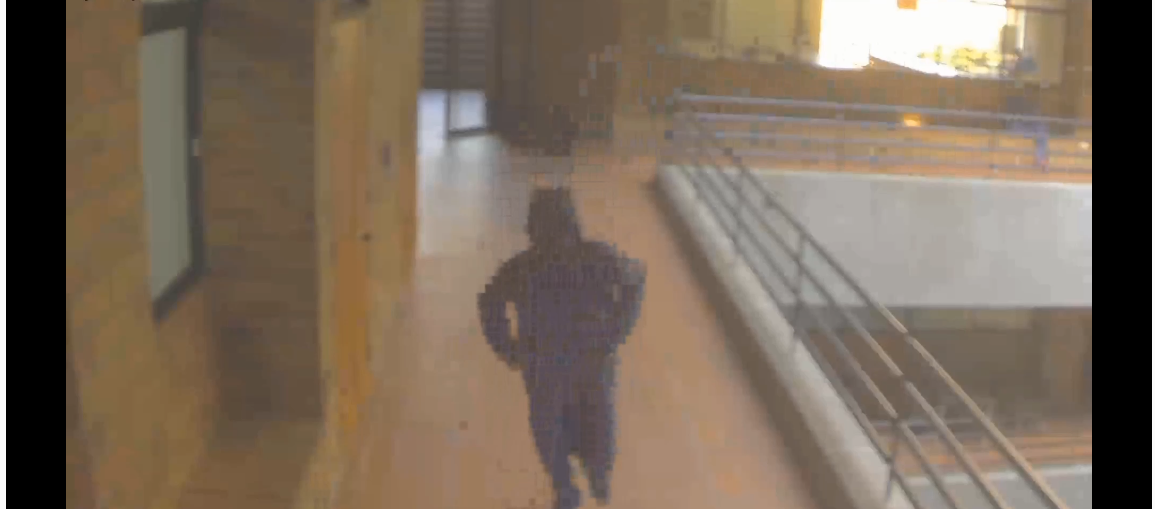
\includegraphics[width=0.19\linewidth]{Person_Running} &
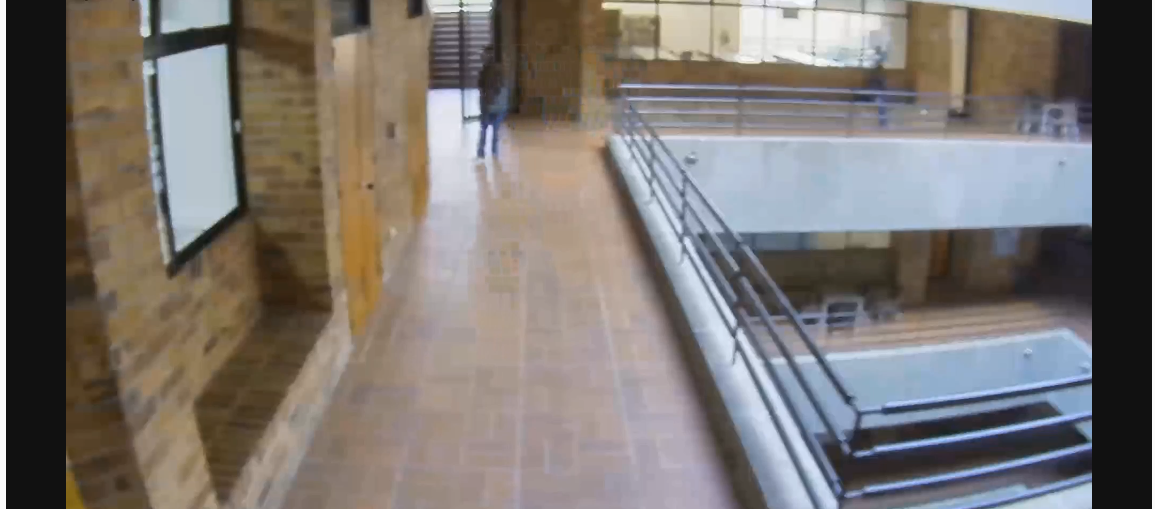
\includegraphics[width=0.19\linewidth]{prowl} &
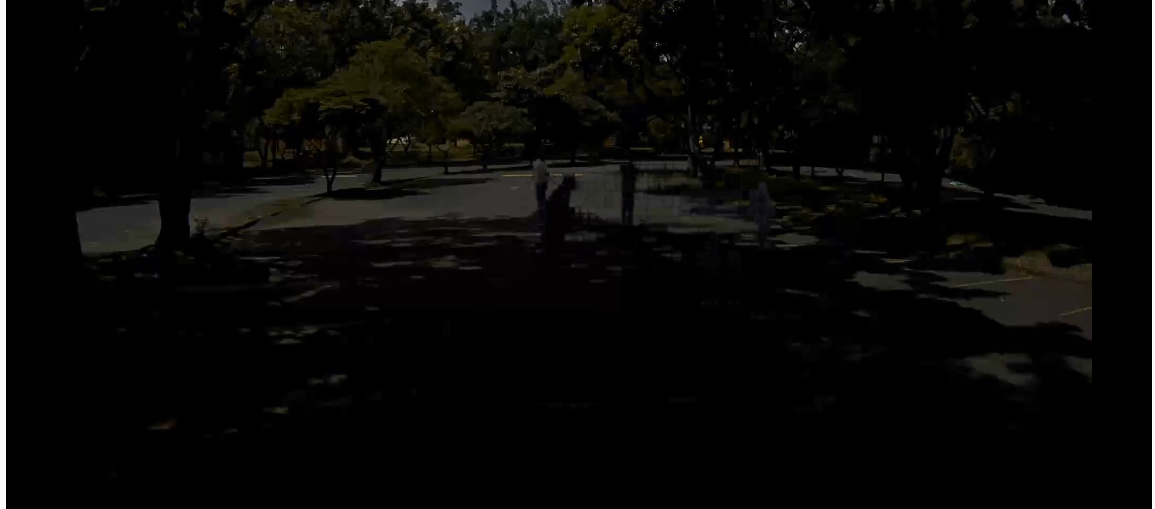
\includegraphics[width=0.19\linewidth]{Robbery_with_Knife} &
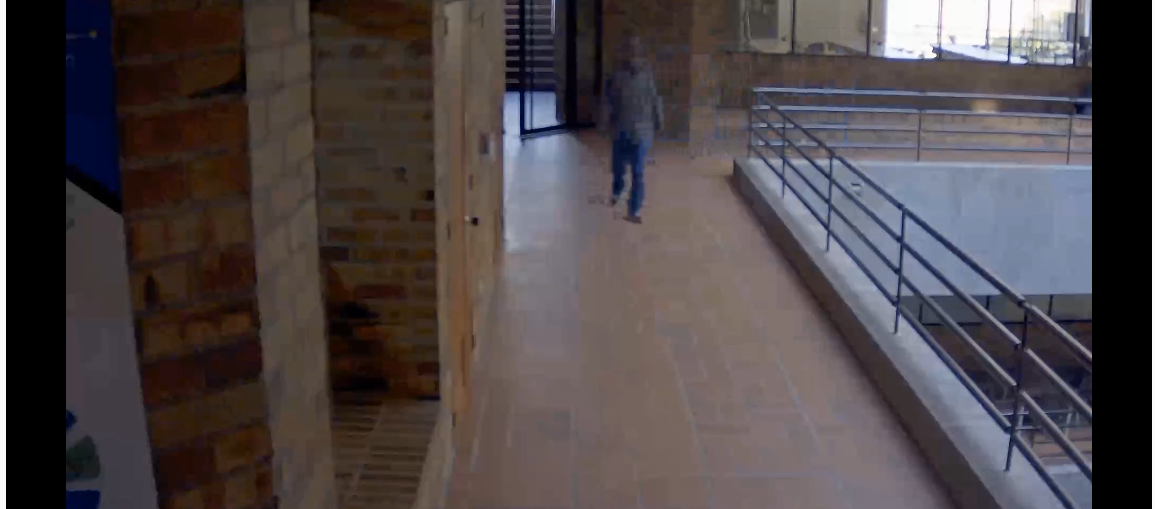
\includegraphics[width=0.19\linewidth]{Walking} \\
\tiny(e) Person Running &
\tiny(f) Prowl &
\tiny(g) Robbery with Knife &
\tiny(h) Walking \\[4pt]
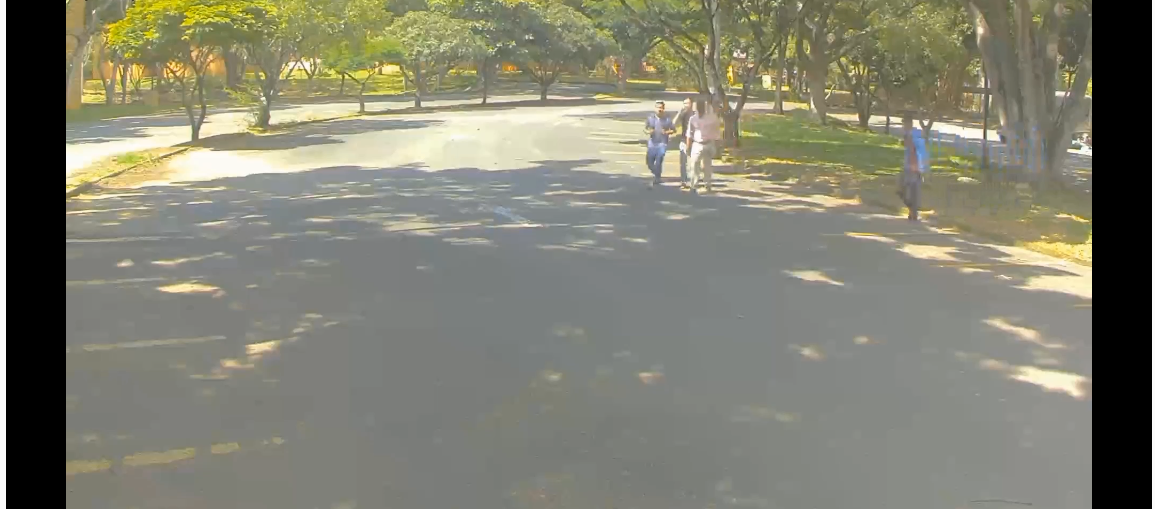
\includegraphics[width=0.19\linewidth]{pristine} &
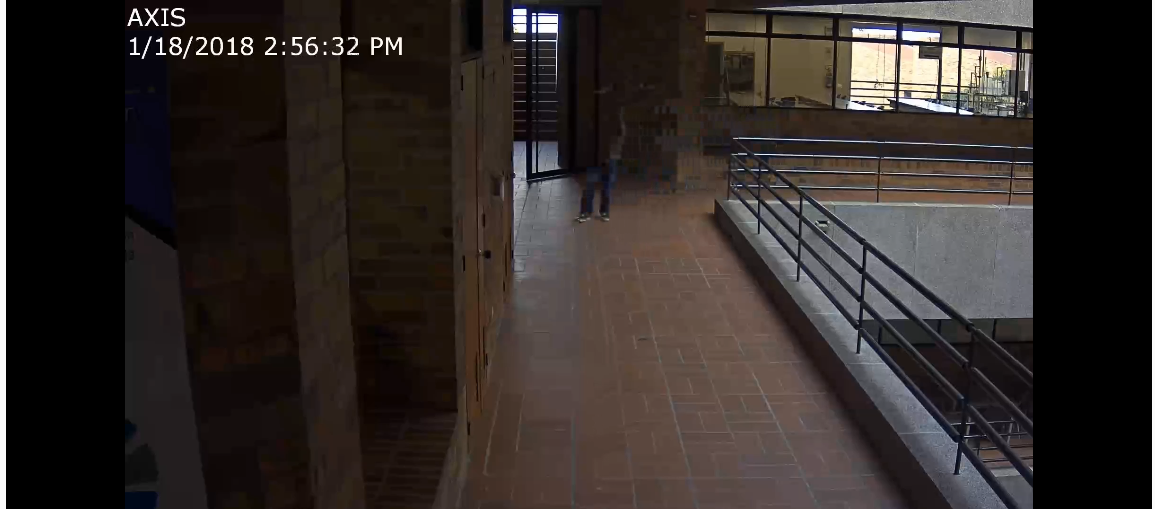
\includegraphics[width=0.19\linewidth]{exposure} &
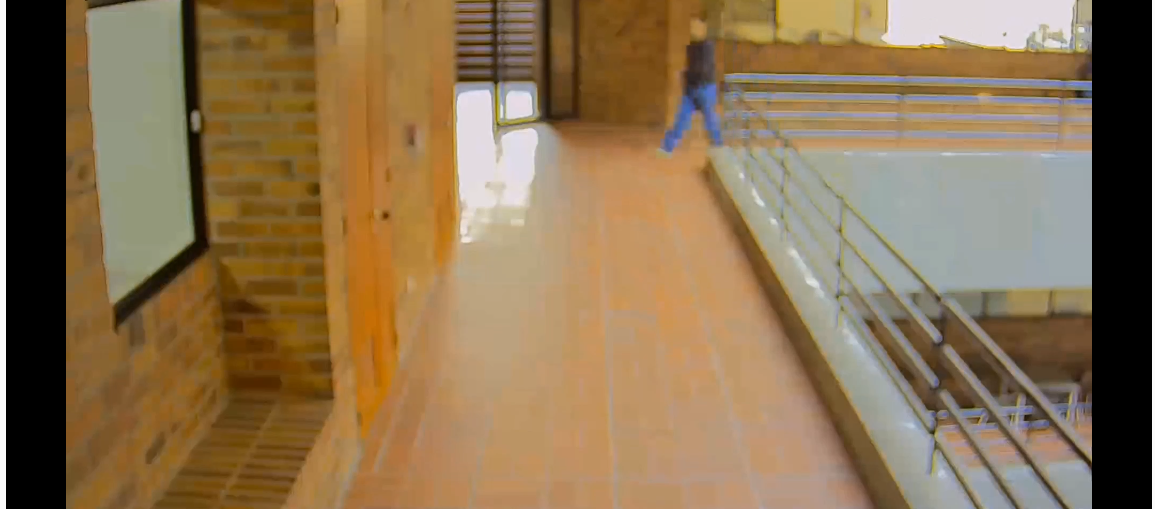
\includegraphics[width=0.19\linewidth]{focus} &
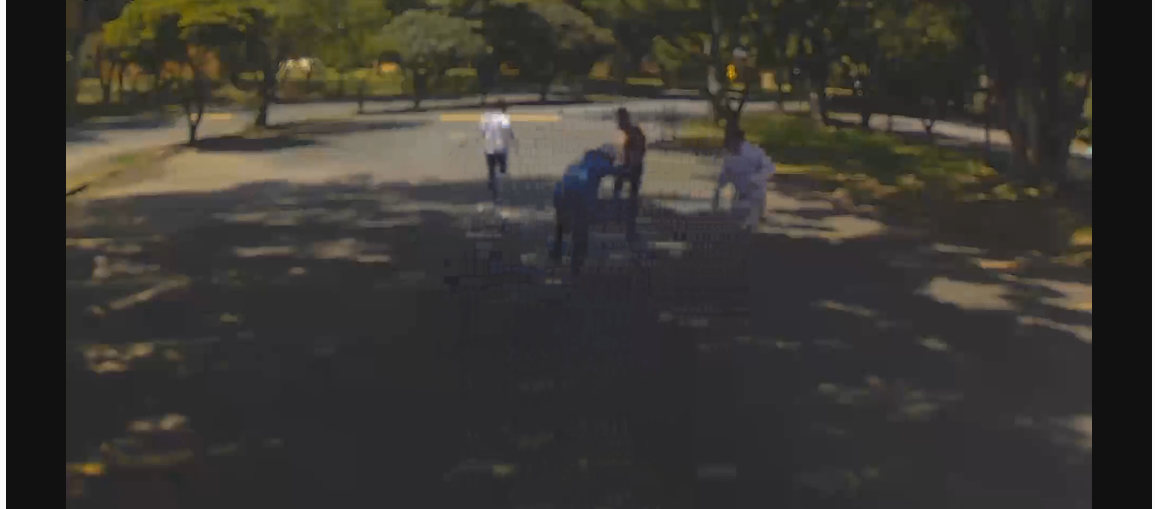
\includegraphics[width=0.19\linewidth]{exfo} \\
\tiny(i) Pristine &
\tiny(j) Exposure &
\tiny(k) Focus &
\tiny(l) Exposure + Focus
\end{tabular}
\caption{\textbf{Representative AD-SVD frames.} (a)--(h) The eight
activity classes, sampled under pristine conditions, forming the target
classes for activity recognition. (i)--(l) The four authentic distortion
conditions; exposure abnormalities and defocus blur degrade the edge and
luminance information required for reliable foreground detection, and
these four conditions form the target classes for distortion
classification.}
\label{fig:examples}
\end{figure}

\paragraph{Research Questions.}

The experimental evaluation is organised around four research
questions, each addressed by a corresponding subsection of
Section~5.

\textbf{RQ1} asks whether adaptive foreground detection improves
trajectory recovery compared with a conventional fixed-threshold
detector; this question is addressed by comparing trajectory yield
across the baseline, ablation, and proposed configurations.
\textbf{RQ2} asks whether improved trajectory recovery translates into
better activity and distortion classification performance; this
question is addressed by comparing classification accuracy across the
same three configurations, allowing the contribution of adaptive
foreground detection to be separated from improvements introduced by
preprocessing and feature representation. \textbf{RQ3} asks which
traditional machine learning classifier provides the strongest
performance on AD-SVD; this question is addressed through a
comprehensive comparison of all evaluated classifiers rather than
reporting only the best-performing model. \textbf{RQ4} asks whether
trajectory-derived motion statistics can classify distortion type
without explicit image-quality analysis; this question is addressed
through distortion classification accuracy and confusion-matrix
analysis under the proposed pipeline.

% ============================================================
\section{Results and Discussion}

This section works through RQ1 to RQ4 in order to test, experimentally, 
the hypothesis set out in Section~1, then draws out what the combined 
results mean for AD-SVD as a benchmark, for the traditional machine 
learning versus deep learning question, and for surveillance practice.

\paragraph{RQ1: Effect of adaptive detection on trajectory recovery.}

Table~\ref{tab:yield} reports trajectory yield for the three 
configurations. Under the fixed-threshold baseline, only 2,083 
of 4,476 videos (46.5\%) produced a usable trajectory; adding 
distortion-aware preprocessing and a richer feature set without 
adaptive detection (the ablation) raises this only modestly, 
to 51.4\%. Adaptive detection raises yield to 99.7\%, and the 
residual 15 failures come from missing source files rather 
than from detection or tracking failure.

This answers RQ1 directly: fixed-threshold foreground detection, 
rather than tracking or feature extraction, is the main factor 
limiting how much of AD-SVD is usable for classification at all, 
and making the detector adaptive closes almost the entire gap on 
its own. Authentic distortions push foreground statistics away 
from a single global operating point in different ways across 
videos, so that a fixed variance threshold that works for some 
clips fails for others; confidence-guided threshold relaxation 
lets the detector respond to each video's own foreground 
statistics instead.

\begin{table}[htbp]
\centering
\caption{\textbf{Trajectory yield by configuration} (of 4,476 videos).}
\label{tab:yield}
\fontsize{8}{9.6}\selectfont
\begin{tabular}{lccl}
\toprule
\textbf{Configuration} & \textbf{Successful videos} & \textbf{Yield} & \textbf{Failure mode} \\
\midrule
Baseline (fixed MOG2) & 2,083 & 46.5\% & Detection failure \\
Ablation (fixed MOG2 + D-A preproc./feat.) & 2,299 & 51.4\% & Detection failure \\
\textbf{Proposed (adaptive MOG2)} & \textbf{4,461} & \textbf{99.7\%} & Missing files only \\
\bottomrule
\end{tabular}
\end{table}

\paragraph{RQ2: Effect on classification performance.}

Table~\ref{tab:activity} reports the best cross-validation result 
(by accuracy, with cross-fold standard deviation) for each configuration. 
The proposed pipeline, classified with LightGBM, reaches 75.5\%$\pm$0.7 
activity accuracy and 97.7\%$\pm$0.5 distortion accuracy on the 
near-complete 4,461-video set, a gain of 6.1 points on activity and 
32.1 points on distortion classification over the best classifier 
on the fixed-threshold baseline (LightGBM, 69.4\%$\pm$2.1 activity; 
XGBoost, 65.6\%$\pm$2.2 distortion).

The ablation, despite using the same distortion-aware preprocessing and a 
feature set of comparable richness (147-dim) to the proposed pipeline, 
performs \emph{worse} than the plain baseline (62.9\%$\pm$2.5 
activity / 60.6\%$\pm$2.4 distortion, best classifier LightGBM in both 
cases), even on its own, slightly larger surviving set of 2,299 videos. 
A paired $t$-test on LightGBM's five cross-validation folds confirms the 
proposed pipeline's gain over the baseline is significant 
($t(4){=}5.5$, $p{=}0.005$ for activity accuracy).

This answers RQ2: enriching preprocessing and features without fixing 
detection does not improve downstream classification accuracy, despite 
modestly improving trajectory yield (46.5\% to 51.4\%), and here it 
actually lowers accuracy relative to the simpler baseline. The 
extra feature dimensions in the ablation are computed from the 
same short, fragmented, low-quality trajectories that a 
fixed-threshold detector produces, so that richer statistics over 
noisier trajectories add variance without adding signal; standardisation 
inside the classification pipeline cannot recover information that 
detection never extracted. The gain we see in the proposed pipeline 
therefore comes from fixing the detection bottleneck itself, not 
from the extra preprocessing or features layered on top of it.

\begin{table}[htbp]
\centering
\caption{\textbf{Classification results, best classifier per configuration} (5-fold cross-validation accuracy, mean $\pm$ std.).}
\label{tab:activity}
\fontsize{8}{9.6}\selectfont
\begin{tabular}{lcccc}
\toprule
\textbf{Configuration} & \textbf{$n$} & \textbf{Best classifier} & \textbf{Activity Acc.} & \textbf{Distortion Acc.} \\
\midrule
Baseline & 2,083 & LightGBM / XGBoost & 69.4\%$\pm$2.1 & 65.6\%$\pm$2.2 \\
Ablation & 2,299 & LightGBM & 62.9\%$\pm$2.5 & 60.6\%$\pm$2.4 \\
\textbf{Proposed} & \textbf{4,461} & \textbf{LightGBM} & \textbf{75.5\%$\pm$0.7} & \textbf{97.7\%$\pm$0.5} \\
\bottomrule
\end{tabular}
\end{table}

\paragraph{RQ3: Classifier comparison.}

Table~\ref{tab:classifiers} reports every classifier evaluated under 
the baseline and proposed configurations.

Under the baseline, the custom Random Forest (implemented from first 
principles) reaches 61.5\%$\pm$2.2 activity / 58.2\%$\pm$3.1 distortion 
accuracy, below the scikit-learn Random Forest (67.7\%$\pm$2.6/67.0\%$\pm$4.2) 
and the boosted models (LightGBM and XGBoost, both above 64\% on both tasks), 
while SVM and KNN trail noticeably (59.3\%$\pm$2.3 and 51.8\%$\pm$3.1 activity 
accuracy, respectively). This spread is small compared with the 6-to-32-point 
gap between the baseline and the proposed configuration in Table~\ref{tab:activity}, 
supporting the conclusion that classifier sophistication matters far less than 
trajectory quality.

Under the proposed configuration, LightGBM and XGBoost are close on distortion 
classification (97.7\%$\pm$0.5 versus 97.5\%$\pm$0.2, overlapping within one 
standard deviation), so we treat the two boosted models as comparable on that 
task; LightGBM's advantage is clearer on activity recognition 
(75.5\%$\pm$0.7 versus 72.3\%$\pm$0.9 for XGBoost and 72.8\%$\pm$1.1 for 
Random Forest). A paired $t$-test over the five cross-validation folds 
confirms LightGBM outperforms XGBoost on every fold ($t(4){=}6.3$, $p{=}0.003$) 
and Random Forest on every fold ($t(4){=}4.0$, $p{=}0.017$) for activity 
recognition. Gradient boosting likely wins on the harder eight-way activity 
task because boosting fits successive corrections to the errors of earlier 
trees on the specific videos that are hardest to separate, while Random 
Forest's independently trained trees simply average over those same errors. 
On the four-way, easier distortion task this advantage mostly disappears, 
which fits with both boosted models levelling out near the achievable 
ceiling once trajectory yield is close to complete.

\begin{table}[htbp]
\centering
\caption{\textbf{Full classifier comparison} (5-fold cross-validation 
accuracy, mean $\pm$ std.). SVM, KNN, and the custom Random Forest were 
evaluated only under the baseline configuration (Section~3).}
\label{tab:classifiers}
\fontsize{8}{9.6}\selectfont
\begin{tabular}{lcccc}
\toprule
& \multicolumn{2}{c}{\textbf{Baseline}} & \multicolumn{2}{>{\columncolor{gray!12}}c}{\textbf{Proposed}} \\
\cmidrule(lr){2-3}\cmidrule(lr){4-5}
\textbf{Classifier} & \textbf{Activity} & \textbf{Distortion} & \cellcolor{gray!12}\textbf{Activity} & \cellcolor{gray!12}\textbf{Distortion} \\
\midrule
Random Forest (sklearn) & 67.7\%$\pm$2.6 & 67.0\%$\pm$4.2 & \cellcolor{gray!12}72.8\%$\pm$1.1 & \cellcolor{gray!12}93.7\%$\pm$0.7 \\
Random Forest (custom) & 61.5\%$\pm$2.2 & 58.2\%$\pm$3.1 & \cellcolor{gray!12}-- & \cellcolor{gray!12}-- \\
SVM (RBF) & 59.3\%$\pm$2.3 & 53.7\%$\pm$2.7 & \cellcolor{gray!12}-- & \cellcolor{gray!12}-- \\
KNN ($k{=}5$) & 51.8\%$\pm$3.1 & 50.1\%$\pm$2.5 & \cellcolor{gray!12}-- & \cellcolor{gray!12}-- \\
XGBoost & 68.3\%$\pm$2.1 & \textbf{65.6\%$\pm$2.2} & \cellcolor{gray!12}72.3\%$\pm$0.9 & \cellcolor{gray!12}97.5\%$\pm$0.2 \\
\textbf{LightGBM} & \textbf{69.4\%$\pm$2.1} & 64.4\%$\pm$1.5 & \cellcolor{gray!12}\textbf{75.5\%$\pm$0.7} & \cellcolor{gray!12}\textbf{97.7\%$\pm$0.5} \\
\bottomrule
\end{tabular}
\end{table}

\paragraph{RQ4: Distortion classification from motion statistics.}

Figure~\ref{fig:confusion} shows the confusion matrices for the proposed 
configuration using the scikit-learn Random Forest (200 trees), which 
reaches 72.8\%$\pm$1.1 activity accuracy (weighted F1 72.7\%$\pm$1.1) 
and 93.7\%$\pm$0.7 distortion accuracy (weighted F1 93.4\%$\pm$0.6); 
LightGBM, the best overall classifier, gives very similar confusion 
patterns with slightly higher per-class accuracy 
(weighted F1 75.5\%$\pm$0.7 activity, 97.7\%$\pm$0.5 distortion, 
closely tracking its accuracy). Focus distortion stays highly 
distinguishable, and with near-complete trajectory coverage the 
distortion classes separate clearly.

This answers RQ4: motion statistics taken purely from trajectories, 
with no explicit image-quality analysis, are enough to classify 
distortion type with high accuracy. Defocus systematically shortens 
tracks, increases fragmentation, and reduces mean speed effects 
measurable reliably across nearly the whole dataset with adaptive 
detection rather than only its most tractable 46.5\%.

\begin{figure}[htbp]
\centering
\begin{tabular}{@{}c@{\hspace{6pt}}c@{}}
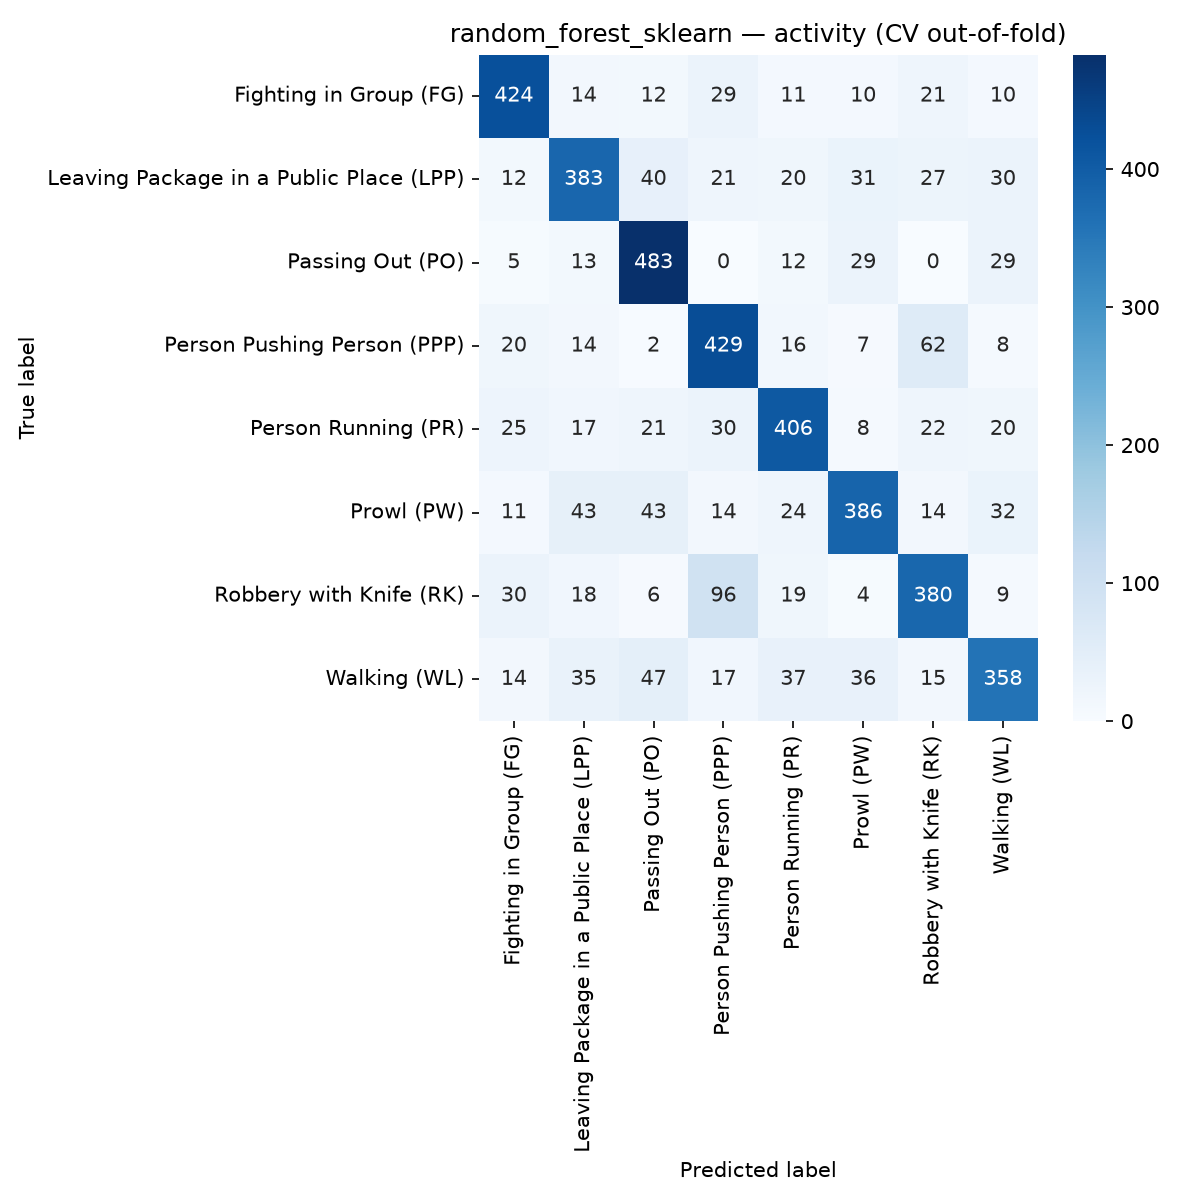
\includegraphics[width=0.47\linewidth]{confusion_activity_groupI_rf} &
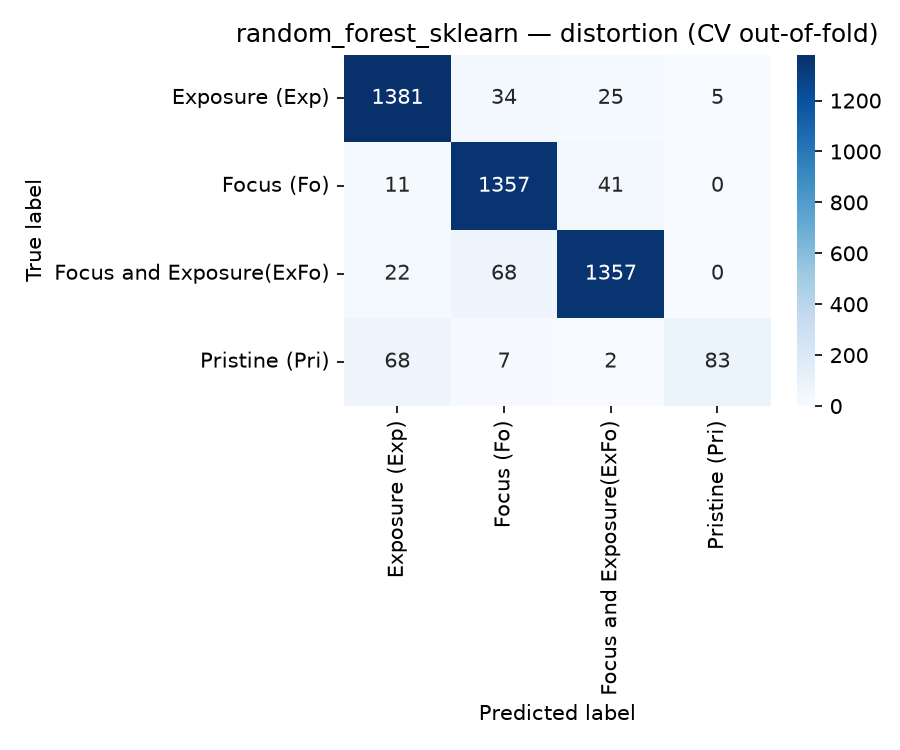
\includegraphics[width=0.47\linewidth]{confusion_distortion_groupI_rf}\\[2pt]
\tiny(a) Activity ($8{\times}8$) &
\tiny(b) Distortion ($4{\times}4$)
\end{tabular}
\caption{\textbf{Confusion matrices, proposed configuration (scikit-learn Random Forest, cross-validation).} (a) Fighting in Group and Prowl are cleanest; Person Pushing Person shows the most confusion with Robbery with Knife, both close-contact activities with visually similar trajectory shapes. (b) Distortion classes are clearly separated once trajectory yield is near-complete.}
\label{fig:confusion}
\end{figure}

\paragraph{Discussion.}

\textbf{Feature importance.} Under the baseline, speed statistics (mean, 
maximum, standard deviation) are the most discriminative features, followed 
by spatial coverage. Under the proposed configuration, the multi-family 
blend means appearance (HOG/LBP) and kinematic descriptors contribute 
alongside trajectory speed statistics; a full per-family importance 
ranking is left to the extended version of this paper.

\textbf{Traditional machine learning versus deep learning.} At AD-SVD's 
current scale (4,476 videos, eight activity classes), trajectory quality 
sets the accuracy ceiling, not classifier expressiveness: the proposed 
pipeline's gain over the baseline comes almost entirely from detection, 
and the ablation shows that adding feature capacity without fixing detection 
can actively hurt accuracy. This supports handcrafted trajectory 
representations as a competitive, data-efficient baseline, since they encode 
motion priors that would otherwise require far more labelled data to 
learn—not evidence that deep learning is inherently worse here, only 
that it is not yet the better-supported choice at this dataset's 
current scale.

\textbf{Surveillance practice.} For deployments recording video under real, 
uncontrolled camera conditions, effort is better spent on the detection 
stage than on the classifier: Table~\ref{tab:activity} shows that adding 
richer features to a weak detector can make accuracy worse, not better, 
while fixing detection alone recovers most of the achievable gain. A 
practitioner seeing poor classification accuracy under authentic 
distortion should therefore check trajectory yield and mask quality 
before tuning the classifier. Because the accuracy ceiling here is 
set by detection rather than by the classifier, a lightweight, 
CPU-only classical pipeline with Adaptive MOG2 is a reasonable choice 
for resource-constrained deployments.

\textbf{AD-SVD as a benchmark.} Detection quality should be checked and 
reported before classification results are compared: two pipelines with 
identical classifiers and similar feature sets can differ by more than 30 
points simply because one recovers usable trajectories from twice as many 
videos. We report yield explicitly in Table~\ref{tab:yield} for this reason, 
and suggest future work on this benchmark do the same.

% ============================================================
\subsection{Controlled ablations and sensitivity analyses}
\label{sec:ablations}

\textcolor{red}{[TODO: fill in after running \texttt{run\_review\_experiments.sh}. Replace every red item. Use the same $\tau$ for all tables.]}

\paragraph{Factorial ablation (detector $\times$ preprocessing $\times$ features).}
To attribute the improvement to adaptive MOG2 rather than to the other changes in the proposed configuration, we run all eight combinations of fixed/adaptive detector, standard/distortion-aware preprocessing, and trajectory-only/221-dimensional features. Figure~\ref{fig:factorial} shows the effect of each factor with the others held fixed, with 95\% bootstrap intervals over videos. \textcolor{red}{[TODO: state the simple effect of the detector at preprocessing=1, features=1 (Group~I minus Ablation~4), the main effects, and any interaction.]}

\begin{figure}[htbp]
\centering
\IfFileExists{images/fig_factorial_activity.png}{\includegraphics[width=0.8\linewidth]{fig_factorial_activity}}{\fbox{\textcolor{red}{PLACEHOLDER: fig\_factorial\_activity.png (run collect\_paper\_figures.py)}}}
\caption{Effect of each factor on activity macro-F1 (differences with 95\% bootstrap CI). The detector effect is shown at every setting of the other two factors.}
\label{fig:factorial}
\end{figure}

\paragraph{Variance-threshold ablation.}
Figure~\ref{fig:threshold} sweeps the MOG2 variance threshold for fixed and adaptive MOG2. The dashed lines are macro-F1 on the videos that survive at every threshold, because yield changes with the threshold; the right panel shows yield per distortion class. \textcolor{red}{[TODO: report the chosen $\tau$, whether any fixed threshold closes the gap to adaptive MOG2, and whether yield differs for Focus versus Pristine.]}

\begin{figure}[htbp]
\centering
\IfFileExists{images/fig_threshold_activity.png}{\includegraphics[width=\linewidth\linewidth]{fig_threshold_activity}}{\fbox{\textcolor{red}{PLACEHOLDER: fig\_threshold\_activity.png (run collect\_paper\_figures.py)}}}
\caption{MOG2 variance-threshold ablation (activity). Left: macro-F1 with 95\% CI (solid) and on the common video subset (dashed). Centre: overall video yield. Right: yield per distortion class. Green dashed line: literature value 16; grey dotted: previous value 25.}
\label{fig:threshold}
\end{figure}

\paragraph{Sensitivity of the adaptive hyperparameters.}
Figure~\ref{fig:sensitivity} varies $q$, $w$, $\tau_r$ and $\tau_{\min}$ one at a time around the defaults. \textcolor{red}{[TODO: describe robustness.]}

\begin{figure}[htbp]
\centering
\IfFileExists{images/fig_sensitivity_activity.png}{\includegraphics[width=\linewidth\linewidth]{fig_sensitivity_activity}}{\fbox{\textcolor{red}{PLACEHOLDER: fig\_sensitivity\_activity.png (run collect\_paper\_figures.py)}}}
\caption{Sensitivity of adaptive MOG2 to $q$, $w$, $\tau_r$ and $\tau_{\min}$ (activity macro-F1, 95\% bootstrap CI). Dashed line: default.}
\label{fig:sensitivity}
\end{figure}

\section{Conclusion}

We reformulated the Authentically Distorted Surveillance Videos (AD-SVD) 
dataset, previously used only for object tracking evaluation, as a supervised 
classification benchmark by introducing activity recognition and distortion-type 
classification tasks, and provided the first comprehensive comparison of 
traditional machine learning classifiers on authentically distorted surveillance 
footage.

Taken together, the results in Section~5 confirm the hypothesis motivating this 
work: detection quality, not classifier sophistication or feature richness, is 
what limits classification accuracy under authentic distortion. A fixed-threshold 
detector leaves 53.5\% of AD-SVD unusable for classification, and enriching 
preprocessing and features without fixing detection does not recover this loss 
and can reduce accuracy. The proposed Adaptive MOG2 raises trajectory yield to 
99.7\% of the dataset, enabling LightGBM to reach 75.5\%$\pm$0.7 activity 
recognition accuracy and 97.7\%$\pm$0.5 distortion classification accuracy 
under stratified 5-fold cross-validation, with XGBoost statistically comparable 
on the distortion task. Under the current dataset size, handcrafted trajectory 
and appearance representations combined with traditional machine learning 
provides a strong, data-efficient baseline for this benchmark.

\paragraph{Limitations.}
Results are reported on a single dataset with a fixed train/test protocol 
(stratified 5-fold cross-validation); generalisation to other surveillance 
settings, camera types, or distortion mixtures has not been tested. Adaptive 
MOG2 was evaluated only on AD-SVD, and its generalisability to other datasets 
with different cameras, scene layouts, and distortion characteristics remains 
to be investigated. Adaptive MOG2 also introduces modest computational 
overhead, since a fraction of frames require a second foreground-extraction 
pass; this is acceptable for offline evaluation but should be optimised for 
high-frame-rate deployments. Our argument against deep learning is based on 
dataset scale and on the trajectory-quality ceiling observed in Section~5, 
not on a completed head-to-head evaluation against a trained end-to-end model.

\paragraph{Future work.}
Future work should focus on stronger trajectory generation before further 
classifier tuning, since Section~5 shows classifier choice contributes far 
less to accuracy than trajectory quality does. A natural next step is 
replacing IoU-Hungarian tracking with Target-Focusing Convolutional 
Regression (TFCR) tracking~\cite{yuan2020learning} to test whether 
stronger trajectory generation gives further gains once detection is 
fixed. Beyond tracking, useful directions include extending the feature 
representation, testing the pipeline on additional authentically 
distorted surveillance datasets, and finding the dataset scale at which 
end-to-end deep video models become competitive with the handcrafted 
representations used here.

This work establishes, to our knowledge, the first systematic benchmark 
for activity and distortion classification on AD-SVD, providing a 
reproducible foundation for evaluating both traditional and deep 
learning approaches under authentic imaging distortions.

% ============================================================
\bibliographystyle{splncs04}
\bibliography{paper_references}

\end{document}